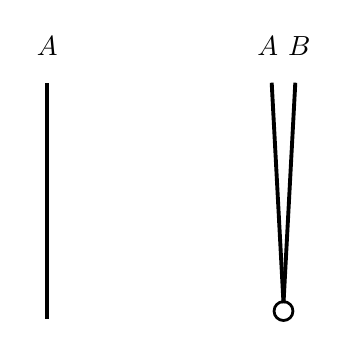
\begin{tikzpicture}[line width=1.4pt]
  % left: single rigid rod A
  \draw (0,0) -- (0,3);
  \node[above] at (0,3.2) {$A$};
  % right: two rods to a pivot ring, splayed
  \draw (2.85,3) -- (3,0.2);
  \draw (3.15,3) -- (3,0.2);
  \draw[line width=1pt] (3,0.1) circle (0.12);
  \node[above] at (2.8,3.2) {$A$};
  \node[above] at (3.2,3.2) {$B$};
\end{tikzpicture}
